\documentclass[11pt]{article}
\usepackage[final]{acl}

\title{Offline Browser-Based ASR with Post-ASR Reconstruction for Under-Supported Languages}

\author{
Cassandre Hamel \quad Vennila Sooben \quad Jean-Christophe Clouatre \quad Imad Benahmed\\
Universit\'e de Montr\'eal\\
\texttt{\{cassandre.hamel, vennila.sooben, jean-christophe.clouatre, imad.benahmed\}@umontreal.ca}
}

\date{IFT 6289 NLP Deep Learning, Winter 2026}

\begin{document}
\twocolumn[
\maketitle
\begin{abstract}
Automatic speech recognition (ASR) remains difficult for languages with limited transcribed audio and productive morphology. This report presents \textit{Shout}, a course project that studies whether lightweight ASR can be made practical in a browser for under-supported languages by combining local Whisper inference, parameter-efficient language adaptation, and post-ASR lexical reconstruction. We focus on Seri (SEI) and Central Puebla Nahuatl (NCX), two Common Voice languages with roughly 11--12 hours of speech each. The repository contains a Vite/Preact browser prototype, Whisper/LoRA training and evaluation scripts, zero-shot baselines, adapted-model metrics, and reconstruction analyses. Zero-shot Whisper-small performs poorly on both languages, with WER 1.351 for SEI and 1.777 for NCX. A SEI LoRA adapter reduces WER to 0.611, and the available NCX adapted evaluation reaches WER 0.154. A simple BK-tree lexical reconstruction step improves zero-shot WER slightly for SEI and more substantially for NCX, but browser-trace metrics show that whole-word correction can also degrade CER and WER when replacements are wrong. The results support local, privacy-preserving ASR as a promising deployment direction, while showing that reconstruction for morphologically complex languages should move beyond whole-word dictionaries toward subword, phonetic, finite-state, or human-in-the-loop correction.
\end{abstract}
\vspace{1em}
]

\section{Introduction}

Large multilingual ASR models have changed the practical baseline for speech transcription, but their gains are unevenly distributed across languages. Systems such as Whisper \citep{radford2023whisper} are trained on large multilingual corpora and can often transcribe unseen languages at a useful level, yet low-resource languages still suffer from limited speaker coverage, scarce labeled audio, domain mismatch, and unstable orthographic conventions. These problems are amplified for morphologically complex and polysynthetic languages, where a single orthographic word may encode information that would be expressed as a phrase or clause in less synthetic languages \citep{gupta2020inuktitut,leferrand2024robust}. In such settings, word-level sparsity makes both training and evaluation difficult: a model can be character-close to the intended output but still receive a high WER, while a lexicon can miss many valid forms.

The project described here asks a practical question: can post-ASR reconstruction make lightweight offline browser ASR practical for under-supported languages? The intended use case is not a server-side benchmark system, but a privacy-preserving browser tool where speech can be recorded, transcribed, and corrected locally. This matters because speech recordings can contain personal, cultural, or community-sensitive content, and because reliable connectivity is not guaranteed in all deployment contexts. A browser application also lowers the barrier for distribution: users do not need to install a Python environment or send audio to a remote service.

The system, named \textit{Shout}, combines three ideas. First, it uses Whisper-style ASR as a strong multilingual foundation. Second, it adapts the model with LoRA adapters, keeping the number of trainable parameters small and allowing one adapter per language \citep{hu2021lora,song2024lorawhisper}. Third, it evaluates a post-processing module that identifies uncertain tokens and maps them to close entries in a language-specific vocabulary using Levenshtein distance. The poster accompanying this report framed the contribution as on-device Whisper inference plus confidence-based lexical correction; the repository scan clarifies that browser worker and confidence plumbing are present, while the most complete reconstruction implementation is the Python evaluation pipeline.

This report makes the following contributions:

\begin{itemize}
    \item it documents the current Shout architecture and repository artifacts;
    \item it reports the available SEI and NCX quantitative results from the project logs;
    \item it analyzes when whole-word BK-tree reconstruction helps or harms ASR metrics;
    \item it identifies deployment and linguistic limitations that should shape future work.
\end{itemize}

\section{Related Work}

\subsection{Low-Resource and Indigenous-Language ASR}

Common Voice provides a multilingual, crowd-sourced corpus for ASR research and has enabled experiments in many languages with limited commercial support \citep{ardila2020common}. However, the existence of a dataset does not remove the core low-resource challenge. Indigenous and under-supported languages often have small speaker pools, heterogeneous recording conditions, uneven prompt coverage, and complex language-specific orthographies \citep{romero2024indigenous}. For polysynthetic languages, ASR difficulty is not only acoustic. Word forms may be sparse, long, and compositionally rich, causing high out-of-vocabulary rates and brittle word-boundary decisions \citep{gupta2020inuktitut,leferrand2024robust}.

This has direct consequences for evaluation. WER treats every segmentation decision as a word-level edit, so it can over-penalize outputs that preserve much of the character content but differ in spacing or affixal detail. CER provides a complementary signal, but it can hide linguistically important boundary errors. The project therefore reports WER and CER together with token and boundary F1 proxies.

\subsection{Whisper, LoRA, and Local Inference}

Whisper is a sequence-to-sequence ASR model trained with weak supervision at large scale \citep{radford2023whisper}. Its multilingual transfer makes it a strong starting point for languages with limited labeled audio, but direct zero-shot use remains unreliable for the languages studied here. Parameter-efficient fine-tuning is a natural response: LoRA freezes the base model and trains small low-rank matrices inside attention projections \citep{hu2021lora}. LoRA-Whisper applies this idea to multilingual ASR and motivates adapter-based expansion without retraining the full model \citep{song2024lorawhisper}.

For local deployment, the browser prototype follows the practical direction opened by whisper.cpp \citep{whispercpp2026}: compact quantized models can run without a cloud service, and model files can be cached locally. The repository's front-end uses Vite and Preact, initializes an ASR worker through Comlink, checks for browser-available Whisper WASM assets, and loads language-specific model files from a local \texttt{/models/} path.

\subsection{Post-ASR Reconstruction}

The reconstruction component is inspired by work that separates recognition from language-specific repair. \citet{diwan2021reduce} propose a reduce-and-reconstruct approach for low-resource phonetic languages, where ASR predicts a simplified representation and a downstream module reconstructs the full form. Shout does not train a reduced representation. Instead, it keeps Whisper's normal text output and applies a lightweight lexical repair layer after decoding. This choice is attractive for browser use because it is simple, interpretable, and fast, but it is also limited: whole-word vocabularies cannot cover the productive morphology that motivates the project in the first place.

\section{Data and Artifacts}

The project uses Common Voice data for Seri and Central Puebla Nahuatl. The poster reports 11 hours, 17 speakers, and 1,615 sentences for SEI; and 12 hours, 41 speakers, and 1,044 sentences for NCX. The available evaluation logs include 452 SEI test clips and 345 NCX test clips for the zero-shot baseline. Table~\ref{tab:data} summarizes the dataset information available in the repository and poster.

\begin{table}[t]
\centering
\scriptsize
\begin{tabular}{lrrrr}
\toprule
Language & Code & Hours & Speakers & Sent.\\
\midrule
Seri & SEI & 11 & 17 & 1,615\\
C. Puebla Nahuatl & NCX & 12 & 41 & 1,044\\
\bottomrule
\end{tabular}
\caption{Common Voice data described in the project poster. The repository logs contain 452 SEI and 345 NCX held-out clips for zero-shot evaluation.}
\label{tab:data}
\end{table}

The repository is organized around three implementation surfaces. The first is the browser application under \texttt{shout/}, which contains the UI, audio recording components, worker bridge, model-loading utilities, confidence utilities, and browser cache helpers. The second is the model experimentation directory \texttt{sei\_ncx\_asr\_model/}, which contains zero-shot evaluation, Whisper+LoRA training, reconstruction, morpheme-F1 evaluation, adapter artifacts, and metrics. The third is \texttt{test/}, which contains browser-trace CSVs and an ASR metrics script used to compare raw and reconstructed outputs.

\begin{table}[t]
\centering
\small
\begin{tabular}{p{0.27\linewidth}p{0.61\linewidth}}
\toprule
Component & Repository evidence\\
\midrule
Browser ASR & Preact app, Comlink worker, WASM/model checks, local model loading, confidence output.\\
LoRA training & Whisper-small fine-tuning script with LoRA rank 32, alpha 64, dropout 0.05, 10 epochs.\\
Reconstruction & Python Levenshtein/BK-style lexical correction with max edit distance 2.\\
Evaluation & WER, CER, token F1, boundary F1, latency, RTF, and reconstruction-rate logs.\\
\bottomrule
\end{tabular}
\caption{Main project artifacts recovered during the repository scan.}
\label{tab:artifacts}
\end{table}

% ============================================================
\section{Evaluation}
\label{sec:evaluation}
% ============================================================

The evaluation is divided into two complementary settings. First, we evaluate the models \emph{off-device}, using the Python evaluation pipeline and held-out Common Voice examples. This setting is useful for comparing recognition quality without the additional constraints of browser execution. Second, we evaluate the system \emph{on-device}, using the browser/WASM prototype from the \texttt{WhisperWasm} branch. This second setting is closer to the intended deployment scenario: local, private, offline transcription for under-supported languages.

The experiments focus on two Common Voice languages: Seri (SEI) and Central Puebla Nahuatl (NCX). Both are low-resource languages in the context of ASR, and both present challenges that are not captured well by English-centered benchmarks. The data consists of roughly 11 hours of Seri speech from 17 speakers and 12 hours of Central Puebla Nahuatl speech from 41 speakers. Since these languages are morphologically rich, a system can be partially correct at the character level while still failing at the word or boundary level. For this reason, we evaluate using four metrics: Word Error Rate (WER), Character Error Rate (CER), token/morpheme F1, and boundary F1.

\subsection{Evaluation Metrics}

WER and CER are the main ASR error metrics. WER measures substitutions, deletions, and insertions at the word level, while CER applies the same idea at the character level. Lower values are better for both metrics. However, WER can be very harsh for polysynthetic or morphologically complex languages: a single long word with a small spelling or segmentation error can count as a full word error. CER therefore provides a useful complementary view.

We also report two F1-style metrics. Token or morpheme F1 measures whether the model recovers the correct lexical units, while boundary F1 measures whether the system places word boundaries correctly. Higher values are better for both. These metrics are especially important because post-ASR reconstruction can sometimes improve word-level matching while damaging character-level fidelity, or vice versa.

\begin{table*}[h]
\centering
\small
\begin{tabular}{lll}
\hline
\textbf{Metric} & \textbf{Direction} & \textbf{Interpretation} \\
\hline
WER & Lower is better & Word-level transcription error \\
CER & Lower is better & Character-level transcription error \\
Token / Morpheme F1 & Higher is better & Recovery of lexical or morpheme-like units \\
Boundary F1 & Higher is better & Correct placement of word boundaries \\
\hline
\end{tabular}
\caption{Evaluation metrics used for both off-device and on-device experiments.}
\label{tab:metrics}
\end{table*}

\subsection{Systems Compared}

The evaluation compares several model configurations. The zero-shot baseline uses a general Whisper model without language-specific adaptation. The monolingual models use language-specific adaptation for a single target language. The joint model uses a shared adaptation setting for both SEI and NCX. Some experiments also include a joint upsampled setting, where the training distribution is adjusted to reduce imbalance between languages.

In addition, the evaluation studies the effect of lexical reconstruction. The reconstruction module uses a language-specific vocabulary and approximate string matching to correct low-confidence ASR tokens. In the intended browser setting, the idea is to identify tokens whose Whisper confidence is below a threshold, then replace them with the nearest valid vocabulary item when the edit distance is small enough. This is designed to be lightweight and compatible with offline browser inference.

% ============================================================
\subsection{Off-Device Evaluation}
% ============================================================

The off-device evaluation measures recognition quality outside the browser. This setting isolates the quality of the ASR model and reconstruction procedure from browser runtime constraints. Figure~\ref{fig:off-device} summarizes the off-device results. The left heatmap reports the absolute performance of zero-shot, monolingual, joint, and joint-upsampled systems. The right heatmap reports the reconstruction effect, where positive values indicate improvement.

\begin{figure}[h]
\centering
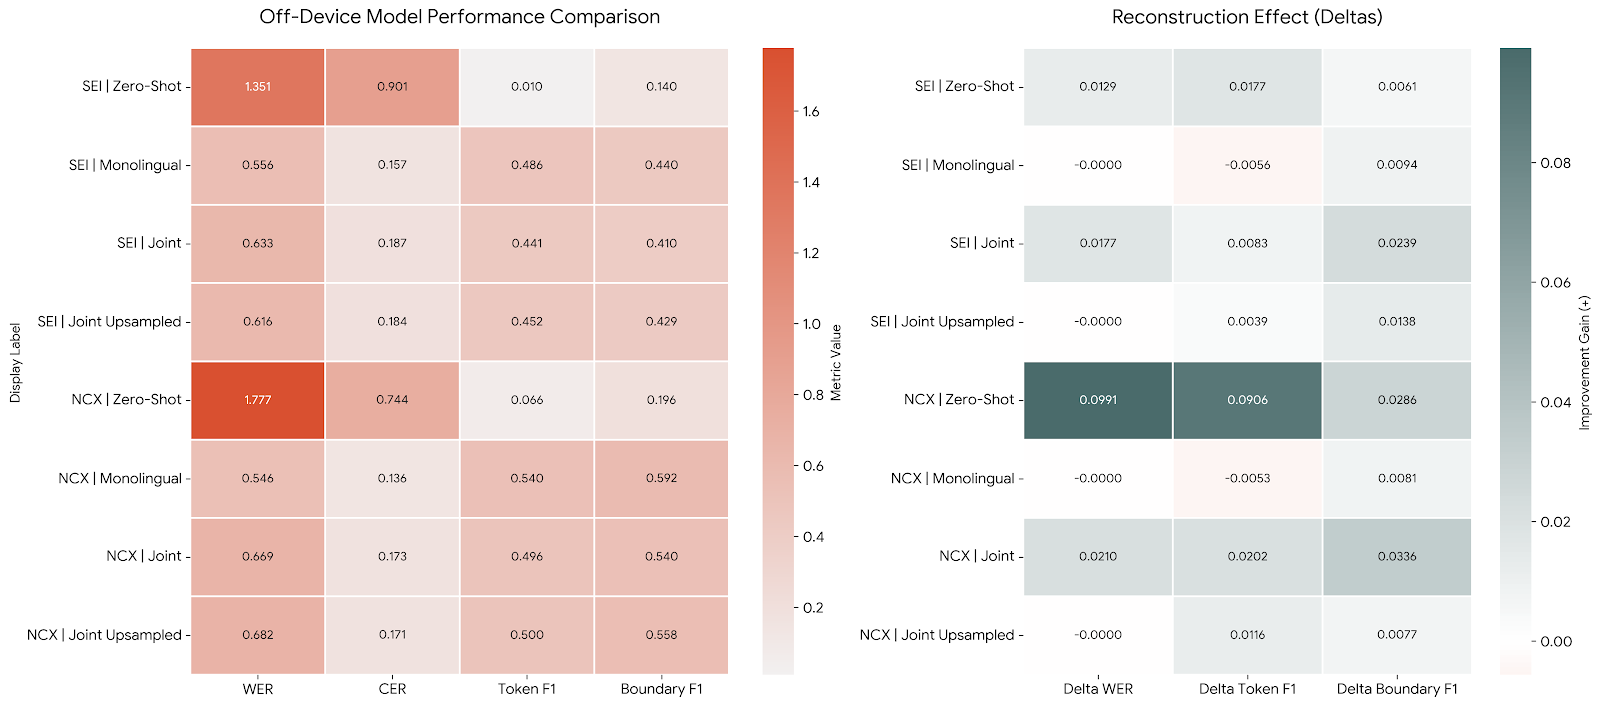
\includegraphics[width=\linewidth]{image8.png}
\caption{Off-device model performance and reconstruction effect for SEI and NCX. Left: absolute WER, CER, token F1, and boundary F1. Right: improvement obtained after reconstruction.}
\label{fig:off-device}
\end{figure}

The off-device results show that zero-shot Whisper is not sufficient for these languages. For SEI, the zero-shot model reaches a WER of 1.351 and a CER of 0.901. For NCX, the zero-shot result is even weaker, with a WER of 1.777 and a CER of 0.744. These values indicate that the model produces many word-level errors and is not reliable as a final transcription system without adaptation.

Language-specific adaptation gives the largest improvement. For SEI, the monolingual model reduces WER from 1.351 to 0.556 and CER from 0.901 to 0.157. It also improves token F1 from 0.010 to 0.486 and boundary F1 from 0.140 to 0.440. For NCX, the monolingual model obtains the strongest overall WER and CER, with WER 0.546 and CER 0.136. It also gives the highest boundary F1, reaching 0.592. These results strongly suggest that monolingual adaptation is the most effective configuration for the target languages.

\begin{table*}[h]
\centering
\small
\begin{tabular}{llcccc}
\hline
\textbf{Lang.} & \textbf{Model} & \textbf{WER} & \textbf{CER} & \textbf{Token F1} & \textbf{Boundary F1} \\
\hline
SEI & Zero-shot & 1.351 & 0.901 & 0.010 & 0.140 \\
SEI & Monolingual & \textbf{0.556} & \textbf{0.157} & \textbf{0.486} & \textbf{0.440} \\
SEI & Joint & 0.633 & 0.187 & 0.441 & 0.410 \\
SEI & Joint upsampled & 0.616 & 0.184 & 0.452 & 0.429 \\
\hline
NCX & Zero-shot & 1.777 & 0.744 & 0.066 & 0.196 \\
NCX & Monolingual & \textbf{0.546} & \textbf{0.136} & \textbf{0.540} & \textbf{0.592} \\
NCX & Joint & 0.669 & 0.173 & 0.496 & 0.540 \\
NCX & Joint upsampled & 0.682 & 0.171 & 0.500 & 0.558 \\
\hline
\end{tabular}
\caption{Off-device model performance. Lower is better for WER and CER; higher is better for token F1 and boundary F1.}
\label{tab:off-device-results}
\end{table*}

The joint and joint-upsampled models improve substantially over zero-shot, but they do not outperform the monolingual adapters. For SEI, the joint model obtains WER 0.633, while the monolingual model reaches 0.556. For NCX, the joint model obtains WER 0.669, compared to 0.546 for the monolingual model. Upsampling slightly improves some metrics, such as SEI WER and boundary F1, but the gains are not enough to close the gap with monolingual adaptation.

This suggests that the two target languages benefit more from specialized adaptation than from a shared adapter. Since the datasets are small and the languages differ linguistically, joint training may introduce interference: the shared model has to represent two different orthographic and acoustic distributions with limited data. Monolingual adapters, in contrast, can specialize more directly to the target language.

\subsubsection{Off-Device Reconstruction Effect}

The reconstruction results are more mixed. In the off-device setting, reconstruction is most useful for the zero-shot models. For NCX zero-shot, reconstruction gives the largest improvement: WER improves by 0.0991, token F1 improves by 0.0906, and boundary F1 improves by 0.0286. For SEI zero-shot, the gains are smaller: WER improves by 0.0129, token F1 by 0.0177, and boundary F1 by 0.0061.

For adapted models, reconstruction gives only small gains and sometimes slightly negative effects. In the SEI monolingual and NCX monolingual settings, WER improvement is essentially zero, while token F1 slightly decreases. This makes sense: once the ASR model is already adapted, its outputs are less noisy, so there are fewer obvious near-miss tokens for reconstruction to fix. At that point, automatic lexical replacement can accidentally replace a valid or nearly valid form with an incorrect vocabulary item.

Overall, the off-device evaluation shows that reconstruction is useful mainly as a repair mechanism for weak ASR outputs. It helps the zero-shot systems, especially NCX, but it is not the main source of improvement. The dominant factor is language-specific adaptation.

% ============================================================
\subsection{On-Device Browser Evaluation}
% ============================================================

The on-device evaluation measures the same general model families inside the browser-based system. This setting is closer to the intended use case: speech is processed locally, using the browser interface and the lightweight model files. Figure~\ref{fig:on-device-absolute} reports the browser model performance before reconstruction, while Figure~\ref{fig:on-device-delta} reports the reconstruction deltas.

\begin{figure}[h]
\centering
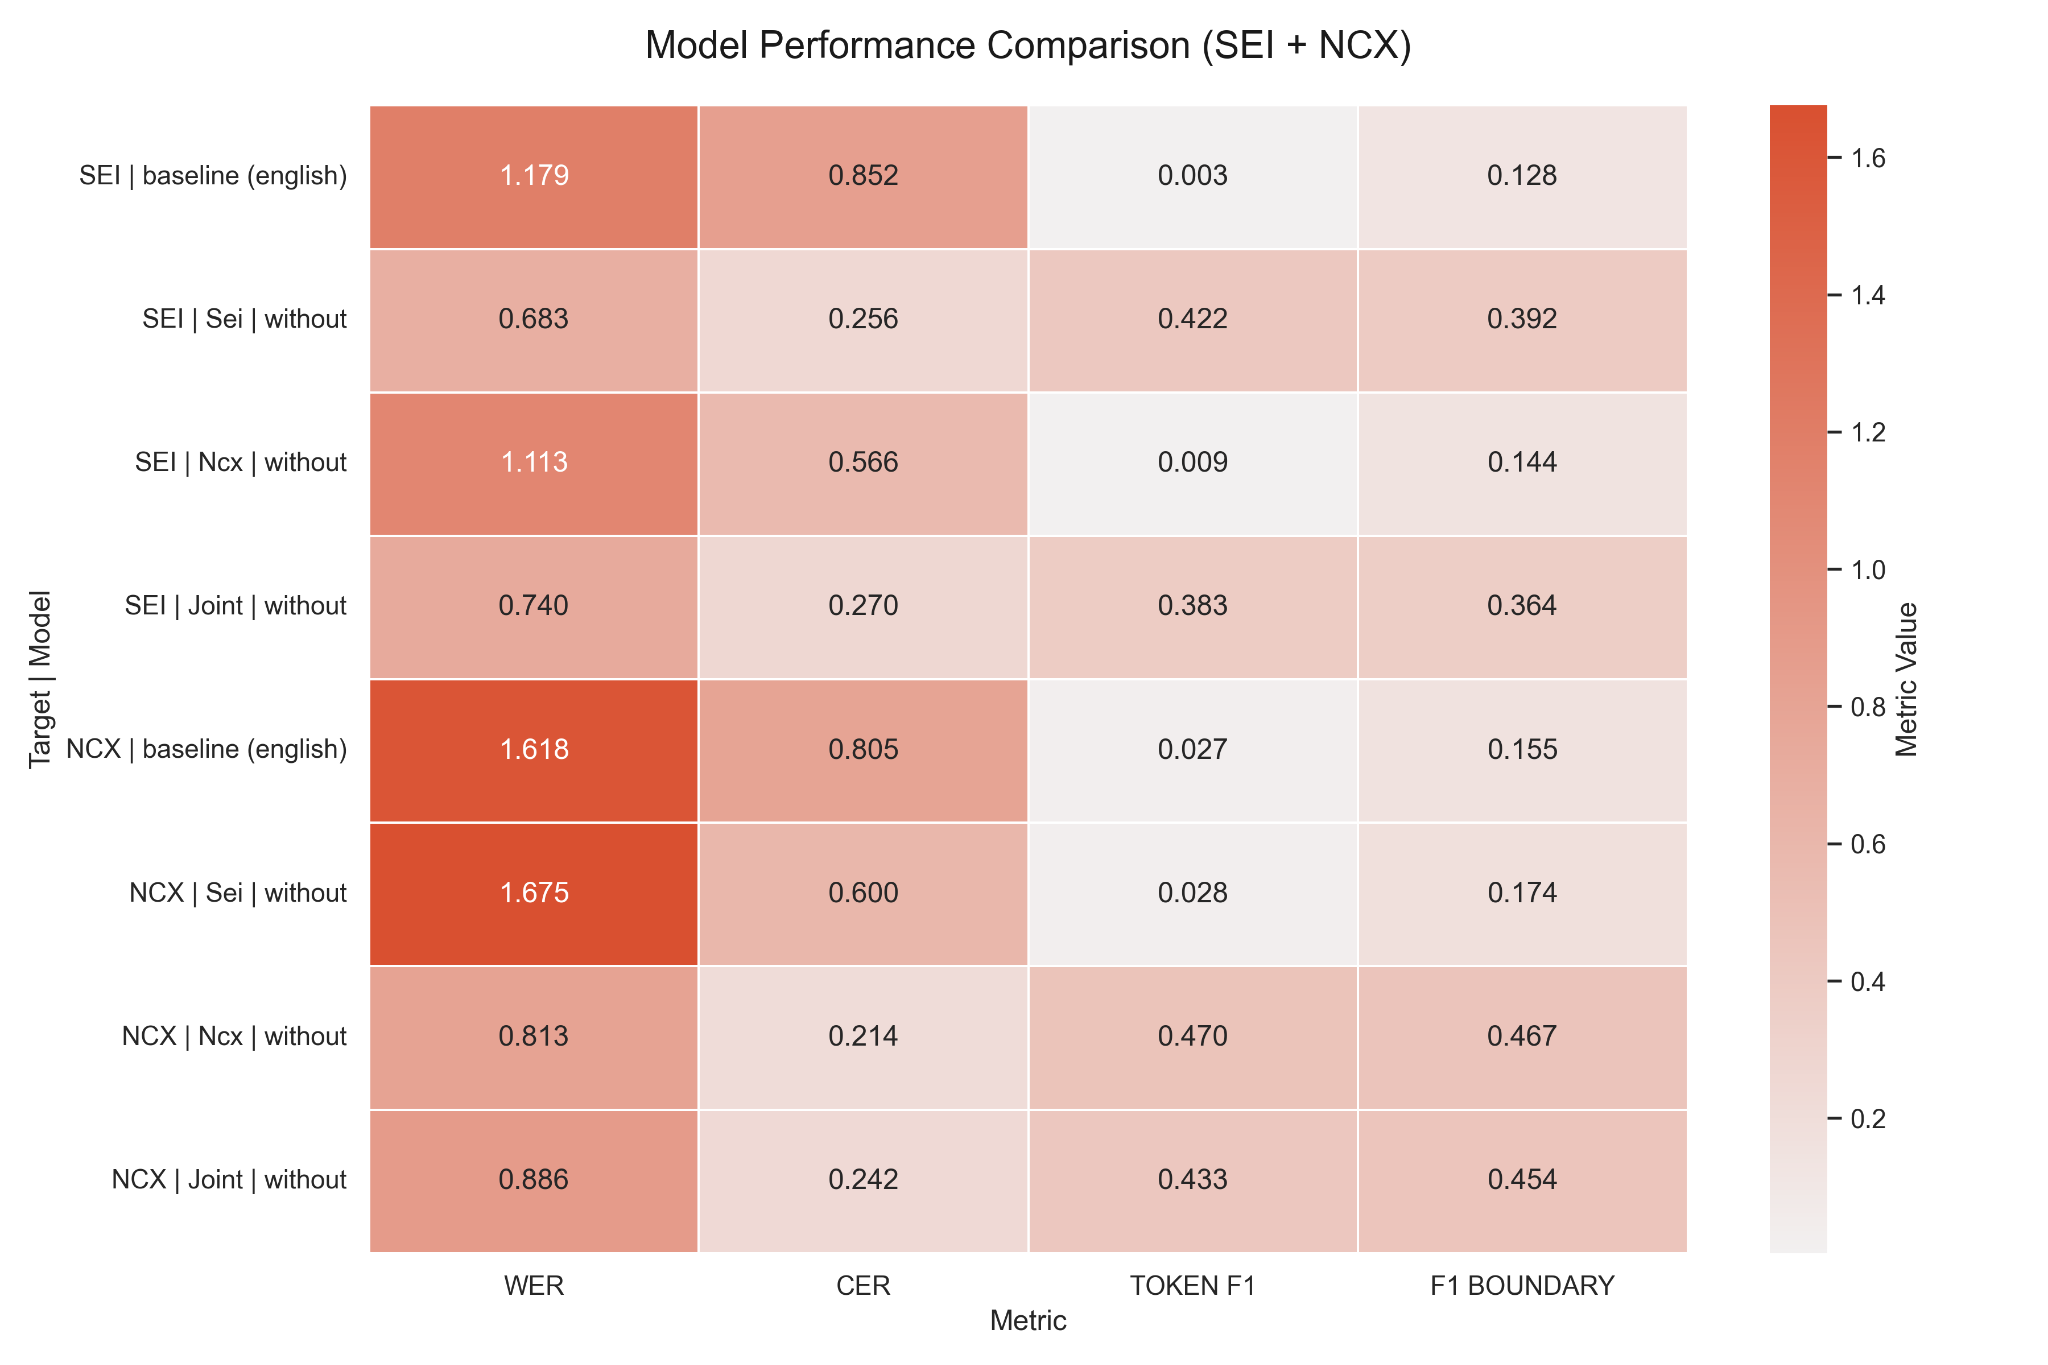
\includegraphics[width=\linewidth]{image5.png}
\caption{On-device/browser model performance for SEI and NCX. The table compares baseline English, language-specific, cross-language, and joint models.}
\label{fig:on-device-absolute}
\end{figure}

The on-device results follow the same broad trend as the off-device results: language-specific models are much stronger than the English baseline or cross-language transfer. For SEI, the English baseline has WER 1.179 and CER 0.852, with almost no token F1. The SEI-specific model reduces WER to 0.683 and CER to 0.256, while increasing token F1 to 0.422 and boundary F1 to 0.392. The SEI joint model is slightly worse than the SEI-specific model, with WER 0.740 and CER 0.270.

For NCX, the English baseline is also weak, with WER 1.618 and CER 0.805. The NCX-specific model gives the best NCX performance, with WER 0.813, CER 0.214, token F1 0.470, and boundary F1 0.467. The NCX joint model is close, with WER 0.886, CER 0.242, token F1 0.433, and boundary F1 0.454, but it still does not surpass the monolingual NCX adapter.

\begin{table*}[h]
\centering
\small
\begin{tabular}{llcccc}
\hline
\textbf{Target} & \textbf{Model} & \textbf{WER} & \textbf{CER} & \textbf{Token F1} & \textbf{Boundary F1} \\
\hline
SEI & English baseline & 1.179 & 0.852 & 0.003 & 0.128 \\
SEI & SEI adapter & \textbf{0.683} & \textbf{0.256} & \textbf{0.422} & \textbf{0.392} \\
SEI & NCX adapter & 1.113 & 0.566 & 0.009 & 0.144 \\
SEI & Joint adapter & 0.740 & 0.270 & 0.383 & 0.364 \\
\hline
NCX & English baseline & 1.618 & 0.805 & 0.027 & 0.155 \\
NCX & SEI adapter & 1.675 & 0.600 & 0.028 & 0.174 \\
NCX & NCX adapter & \textbf{0.813} & \textbf{0.214} & \textbf{0.470} & \textbf{0.467} \\
NCX & Joint adapter & 0.886 & 0.242 & 0.433 & 0.454 \\
\hline
\end{tabular}
\caption{On-device/browser model performance before reconstruction.}
\label{tab:on-device-results}
\end{table*}

The browser results also show that cross-language transfer is unreliable. Using the NCX model on SEI gives WER 1.113, which is only slightly better than the English baseline and far worse than the SEI-specific model. Using the SEI model on NCX gives WER 1.675, which is even worse than the English baseline. This confirms that the adapters learn language-specific properties rather than a general correction strategy that transfers cleanly across the two languages.

\subsubsection{On-Device Reconstruction Effect}

\begin{figure}[h]
\centering
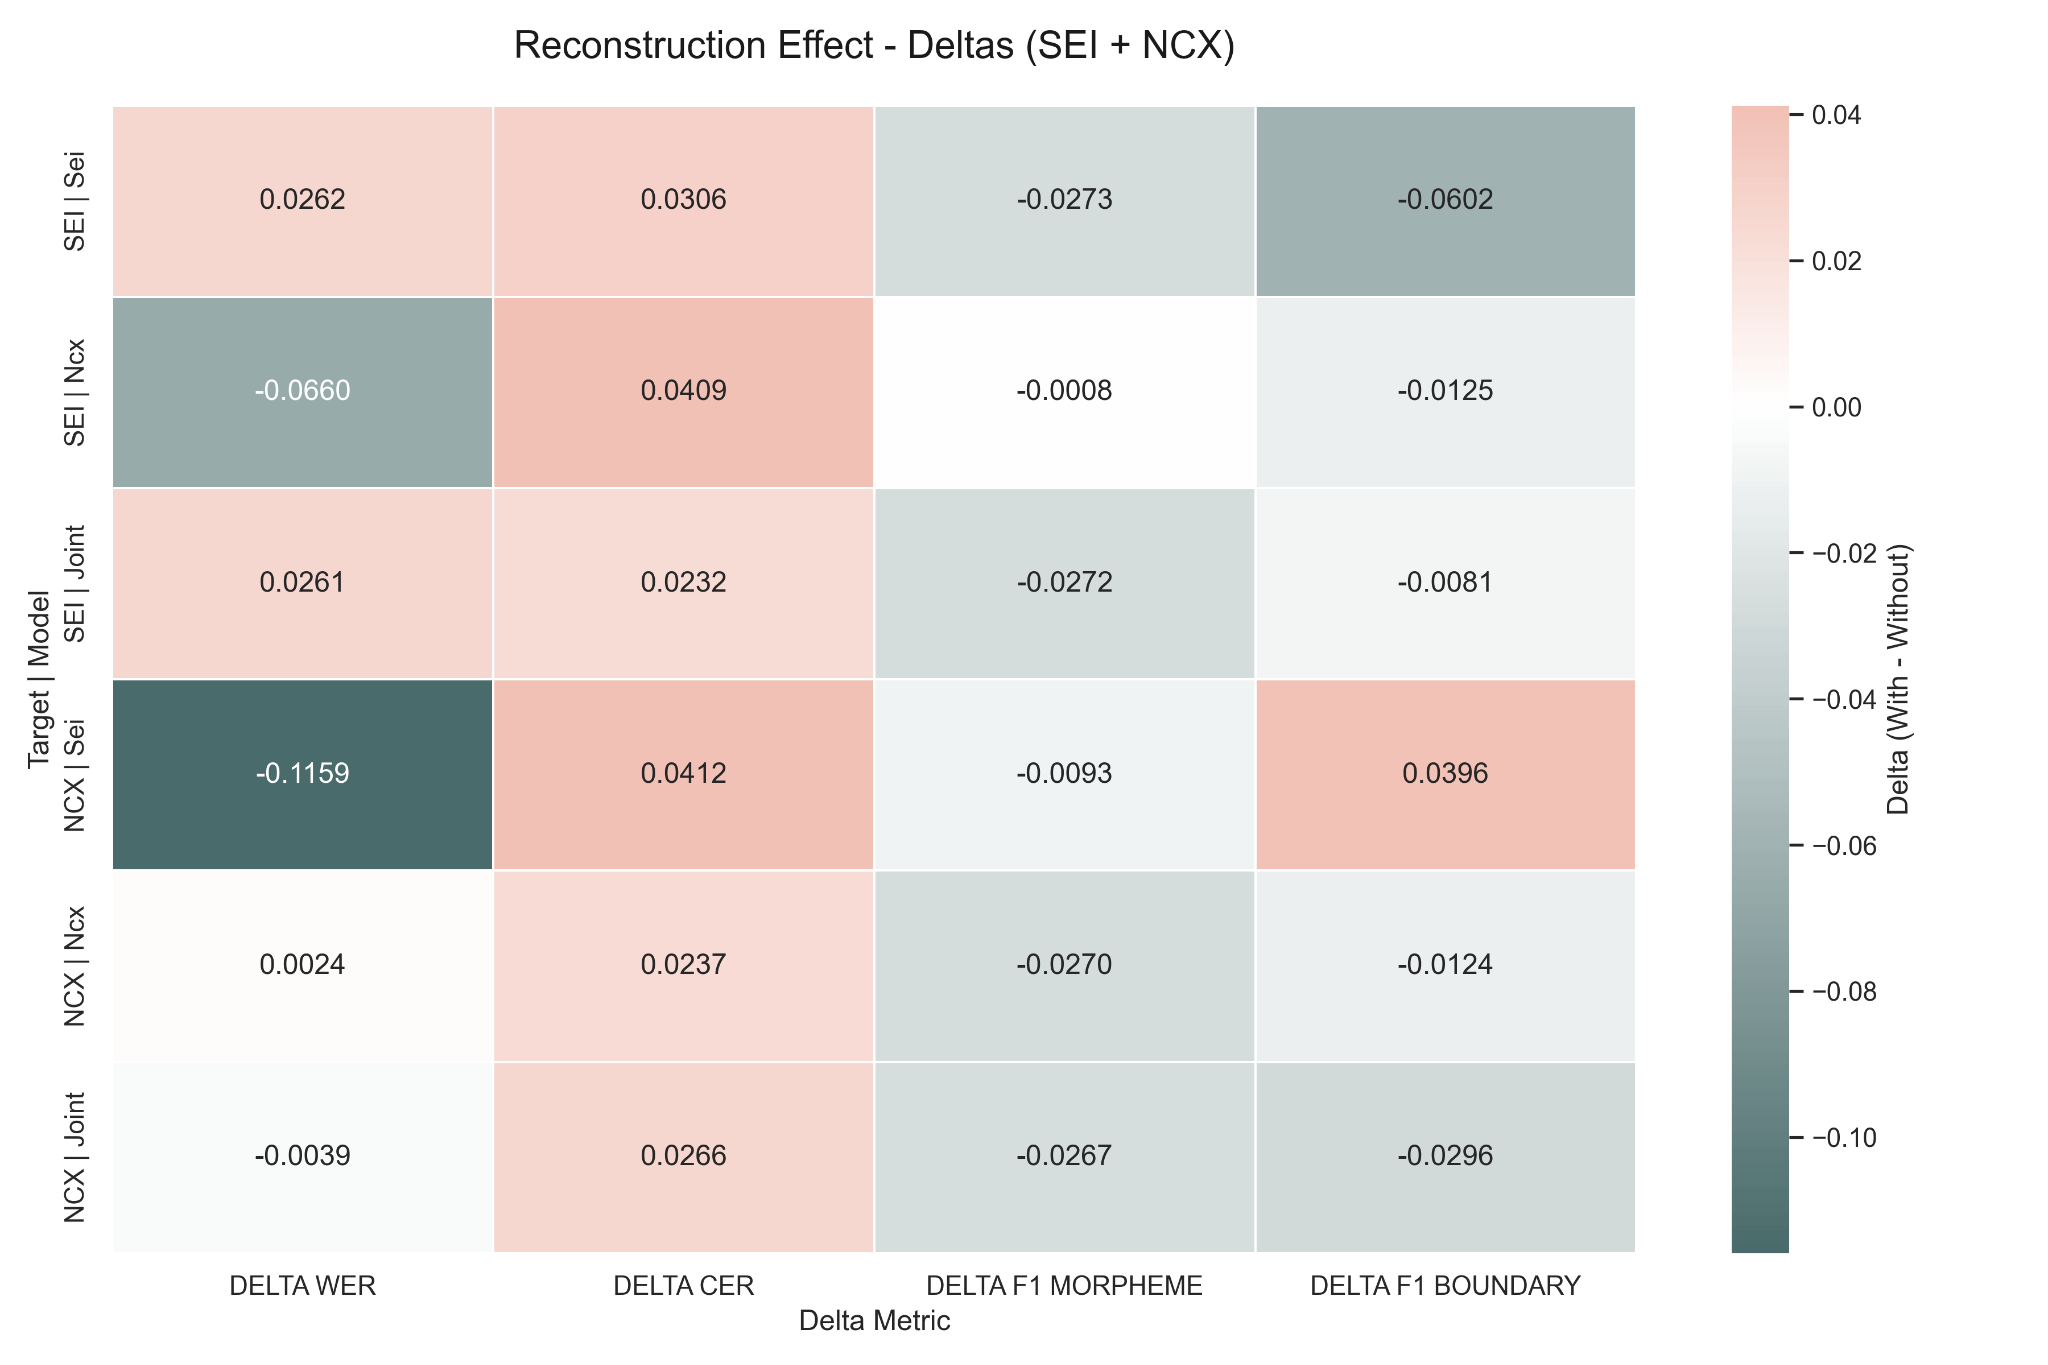
\includegraphics[width=\linewidth]{image1.png}
\caption{On-device/browser reconstruction effect. Deltas are computed as reconstructed output minus output without reconstruction. For WER and CER, negative deltas are better; for F1 metrics, positive deltas are better.}
\label{fig:on-device-delta}
\end{figure}

The browser reconstruction results are mixed and sometimes negative. For WER, reconstruction helps in some cross-language or weaker settings. For example, on SEI with the NCX adapter, WER decreases by 0.0660. On NCX with the SEI adapter, WER decreases by 0.1159. However, these are also settings where the base transcription is poor, so reconstruction has more obvious errors to correct.

For the strongest monolingual models, reconstruction does not consistently help. On SEI with the SEI adapter, WER increases by 0.0262 and CER increases by 0.0306. On NCX with the NCX adapter, WER increases slightly by 0.0024 and CER increases by 0.0237. These changes indicate that reconstruction can damage otherwise good outputs by forcing them toward a limited vocabulary.

The CER results are especially important. Almost every condition shows a positive CER delta, meaning character-level error becomes worse after reconstruction. This suggests that the lexical correction step may replace a token with a dictionary word that is valid in isolation but not actually closer to the reference. In morphologically rich languages, this is a serious limitation: a word-level vocabulary cannot cover all valid inflected or derived forms, so the nearest known word is not always the correct word.

The F1 metrics also show instability. Morpheme/token F1 often decreases after reconstruction, especially for SEI and joint settings. Boundary F1 sometimes improves, such as in the NCX target with the SEI adapter, but it also decreases in several other cases. Therefore, reconstruction should not be interpreted as a universal improvement step. It is better understood as a risky post-processing module whose usefulness depends on the quality of the ASR output, the confidence threshold, and the coverage of the language vocabulary.

% ============================================================
\subsection{Discussion}
% ============================================================

The main conclusion from both off-device and on-device evaluation is that language adaptation matters more than reconstruction. Zero-shot Whisper and the English baseline perform poorly on both SEI and NCX. This is expected because the target languages are under-supported and differ strongly from the high-resource languages that dominate general ASR training. Monolingual adapters provide the largest and most consistent improvements across WER, CER, token F1, and boundary F1.

The second conclusion is that joint training is useful but not optimal. Joint adapters clearly improve over zero-shot or English-only baselines, but they do not surpass monolingual adapters. This is visible in both evaluation settings. For example, off-device SEI WER is 0.556 with the monolingual model and 0.633 with the joint model. On-device NCX WER is 0.813 with the NCX adapter and 0.886 with the joint adapter. The result suggests that, for small low-resource datasets, adapter specialization is more effective than sharing a single adapter across typologically different languages.

The third conclusion is that reconstruction has a narrow useful region. It helps most when the ASR output is weak but close to valid vocabulary items. This explains why the off-device zero-shot NCX system receives the largest reconstruction gain. However, when the ASR model is already adapted, reconstruction can introduce new errors. The most common failure mode is over-correction: the system replaces a token with the nearest vocabulary item even when the original token was acceptable or when the nearest item is not the intended word. This is why CER often worsens after reconstruction in the browser results.

It is also important to interpret the reconstruction results in the context of the method used. The current reconstruction module is intentionally simple: it relies on a BK-tree and Levenshtein distance over a fixed word vocabulary. This makes it lightweight and easy to run locally, but it is also an unreliable correction strategy for morphologically complex languages. The nearest word in edit-distance space is not necessarily the intended word, and many valid forms may be missing from the vocabulary entirely. Therefore, the weak reconstruction results are not surprising. They do not necessarily show that post-ASR reconstruction is a bad direction; rather, they show that a naive whole-word BK-tree approach is not strong enough on its own.

A more advanced reconstruction module could still be highly useful. Future work should move beyond whole-word dictionary lookup toward methods that better match the structure of the target languages. Possible directions include subword-based reconstruction with byte-pair encodings or other unsupervised units, phonetic or IPA-based intermediate representations, rule-based finite-state transducers, and human-in-the-loop correction. These approaches would reduce the risk of forcing the output toward an incorrect dictionary word while still preserving the main advantage of reconstruction: improving noisy ASR output without retraining the full model. In that sense, the current reconstruction results should be seen as a lower-bound baseline for a much richer correction module.

\section{Ethics Statement}

ASR for Indigenous and under-supported languages requires more than technical accuracy. Offline inference reduces privacy risk because audio can stay on the user's device, but data collection, model training, and deployment must still respect consent, licensing, community data governance, and the purposes for which speakers contributed recordings. Automatic correction should be auditable and reversible, especially when outputs may be used for documentation, education, or community archives. The system should support human expertise rather than replacing it, and future evaluation should include community-centered feedback.

\section{Conclusion}

Shout investigates offline browser-based ASR for under-supported languages through Whisper inference, LoRA adaptation, and post-ASR reconstruction. The available results show that zero-shot Whisper-small is insufficient for SEI and NCX, while language adaptation provides large gains. BK-tree lexical reconstruction can improve zero-shot outputs, especially for NCX, but it is not reliable enough as a general correction strategy and can degrade browser-trace metrics. The most promising path is therefore a hybrid one: keep the privacy and accessibility benefits of local browser inference, use language-specific adapters for core recognition quality, and replace whole-word automatic repair with more linguistically aware, thresholded, and user-controllable reconstruction.

\section*{Acknowledgments}

This project was supervised within IFT 6289 NLP Deep Learning, Winter 2026. The implementation builds on Whisper, whisper.cpp, LoRA, PEFT, Hugging Face tooling, and Common Voice. We thank the Seri and Nahuatl language communities whose recordings make this work possible.

\bibliographystyle{plainnat}
\bibliography{references}

\clearpage
\onecolumn
\appendix

\section{Poster Annexe}

The attached project poster is included as an annexe for reference. It summarizes the motivation, dataset, pipeline, threshold analysis, and high-level conclusions presented to the course instructor.

\begin{center}
\includegraphics[width=\textwidth,height=0.82\textheight,keepaspectratio]{assets/poster_presentation.pdf}
\end{center}

\section{Additional Browser Trace Summary}

\begin{table}[t]
\centering
\small
\begin{tabular}{llrrrr}
\toprule
Lang. & Output & Rows & WER & CER & Avg. RTF\\
\midrule
SEI & Raw ASR & 100 & 1.171 & 0.905 & 1.66\\
SEI & Final text & 100 & 1.171 & 0.909 & 1.66\\
NCX & Raw ASR & 100 & 0.929 & 0.505 & 3.49\\
NCX & Final text & 100 & 0.934 & 0.518 & 3.49\\
\bottomrule
\end{tabular}
\caption{Browser-trace metrics from \texttt{test/asr\_metrics\_out/summary.json}. These rows are separated from the main results because they evaluate exported traces rather than the full held-out Common Voice prediction files.}
\end{table}

\end{document}
